% ============================================================
% INTEGRATION LOG — Team 0109D — 04.3_Integration
% ============================================================
\documentclass[12pt, letterpaper]{article}
\usepackage[margin=0.5in]{geometry}
\usepackage[T1]{fontenc}
\usepackage[scaled=1]{helvet}
\renewcommand{\familydefault}{\sfdefault}
\usepackage[utf8]{inputenc}
\usepackage{graphicx}
\usepackage{booktabs}
\usepackage{tabularx}
\usepackage{float}
\usepackage{caption}
\usepackage{hyperref}
\usepackage{enumitem}
\usepackage{xcolor}
\usepackage{titlesec}

\titleformat{\section}{\large\bfseries}{\thesection}{0.6em}{}
\titleformat{\subsection}{\normalsize\bfseries}{\thesubsection}{0.5em}{}
\titlespacing*{\section}{0pt}{8pt}{3pt}
\titlespacing*{\subsection}{0pt}{6pt}{2pt}
\setlist{nosep, leftmargin=1.2em, itemsep=1pt}
\captionsetup{font=small, skip=3pt, labelfont=bf}
\hypersetup{colorlinks=true, urlcolor=blue!60!black}
\graphicspath{{../images/}}
\setlength{\parskip}{3pt}
\setlength{\parindent}{0pt}

\begin{document}

\begin{center}
{\LARGE\textbf{Systems Integration \& Debugging Log}}\\[2pt]
{\normalsize Team 0109D \quad$\vert$\quad ESC204 --- Praxis III \quad$\vert$\quad Winter 2026}
\end{center}
\noindent\rule{\textwidth}{0.6pt}\vspace{4pt}

\section{Integration Timeline}

\begin{table}[H]
\centering\small
\caption{Chronological integration sequence.}
\begin{tabularx}{\textwidth}{@{}l l X@{}}
\toprule
\textbf{Date} & \textbf{Milestone} & \textbf{Outcome} \\
\midrule
Mar 9--13 & Iter.\,1: DC motor + breadboard & Failed: no positional dead reckoning \\
Mar 16--17 & Iter.\,2: DC motor + H-Bridge & Failed: voltage drop $\rightarrow$ stall/jitter \\
Mar 19--20 & Final: Nema\,17 + A4988 assembled & Successful: mm-precise stepping \\
Mar 20 & Power isolation + thermal tuning & Brownouts resolved; VREF set to 50\% \\
Mar 23--25 & Full systems integration on track & Deadzone compensation; firmware upgrade \\
Mar 25 & 2-minute endurance test & Passed: zero stalling, belt stable, thermal OK \\
\bottomrule
\end{tabularx}
\end{table}

\section{Detailed Integration Changes}

\subsection{Change 1: Motor Substitution (DC $\rightarrow$ Stepper)}

The initial drivetrain used a direct-drive DC motor. During integration testing, the DC motor could not perform accurate dead reckoning---time-based movement was unreliable due to variable friction from the belt and changing carriage mass. The system was replaced with a Nema\,17 stepper motor (1.8$^\circ$/step, 200 steps/rev), which provides exact step-count positioning at 0.2\,mm/step via the GT2 belt and 20-tooth pulley.

\textit{Reference Artifact:} \texttt{DC\_Motor\_Breadboard\_Iteration1.jpeg}

\subsection{Change 2: Driver Architecture (H-Bridge $\rightarrow$ A4988)}

An L298N H-Bridge was initially used to drive the DC motor. Under the mass of the carriage and friction of the continuous belt, the H-Bridge suffered extreme voltage drops, resulting in motor stalling and severe jitter. The entire driver architecture was replaced with an A4988 stepper driver and screw-terminal power distribution blocks, eliminating jitter and providing micro-stepping torque control.

\textit{Reference Artifacts:} \texttt{HBridge\_Motor\_Iteration2.jpeg}, \texttt{Stepper\_A4988\_ScrewTerminals\_Final.jpeg}\\
\textit{Video of jitter failure:} \href{https://drive.google.com/drive/folders/1wNK_jYUvHXoMne_cIdYbAIURdvYpuG-J}{[Google Drive]}

\subsection{Change 3: Power Segregation}

Initial integration revealed that pulling high continuous current for the Nema\,17 caused logic brownouts when the motor and Pico shared a power rail. The system was physically segregated: Pico logic operates on an isolated 5\,V USB source (providing clean 3.3\,V to the A4988 $V_{DD}$), while the motor operates on a dedicated 12\,V DC wall adapter routed to $V_{MOT}$.

\subsection{Change 4: Thermal Tuning}

During continuous operation testing, the A4988 driver entered thermal shutdown. The current-limiting potentiometer ($V_{REF}$) was manually calibrated to approximately 50\% capacity. This caps the current to prevent overheating while maintaining sufficient holding and driving torque for the carriage and attached air hose.

\subsection{Change 5: Firmware State-Machine Upgrade}

The CircuitPython firmware was upgraded from simple \texttt{time.sleep()} delays to a reactive, polling-based state machine. The code now actively monitors GP5 and GP6 via internal pull-up resistors. When a limit switch is driven LOW, the A4988 DIR pin reverses instantly rather than waiting for a predefined loop to finish. This guarantees the carriage cannot overrun the track endpoints and damage the timing belt.

\textit{Reference Artifact:} \texttt{firmware/code.py}

\subsection{Change 6: Deadzone Compensation}

During final assembly, we discovered the physical limit switches occupy approximately 2\,cm of track space at each end, creating a mechanical ``deadzone'' where the nozzle cannot reach. To compensate, the nozzle was intentionally mounted with a 2\,cm overhang on each side of the carriage, guaranteeing 100\% surface clearing coverage despite the reduced mechanical travel limits.

\section{Debugging Evidence}

\begin{figure}[H]
\centering
\begin{minipage}[t]{0.30\textwidth}
\centering
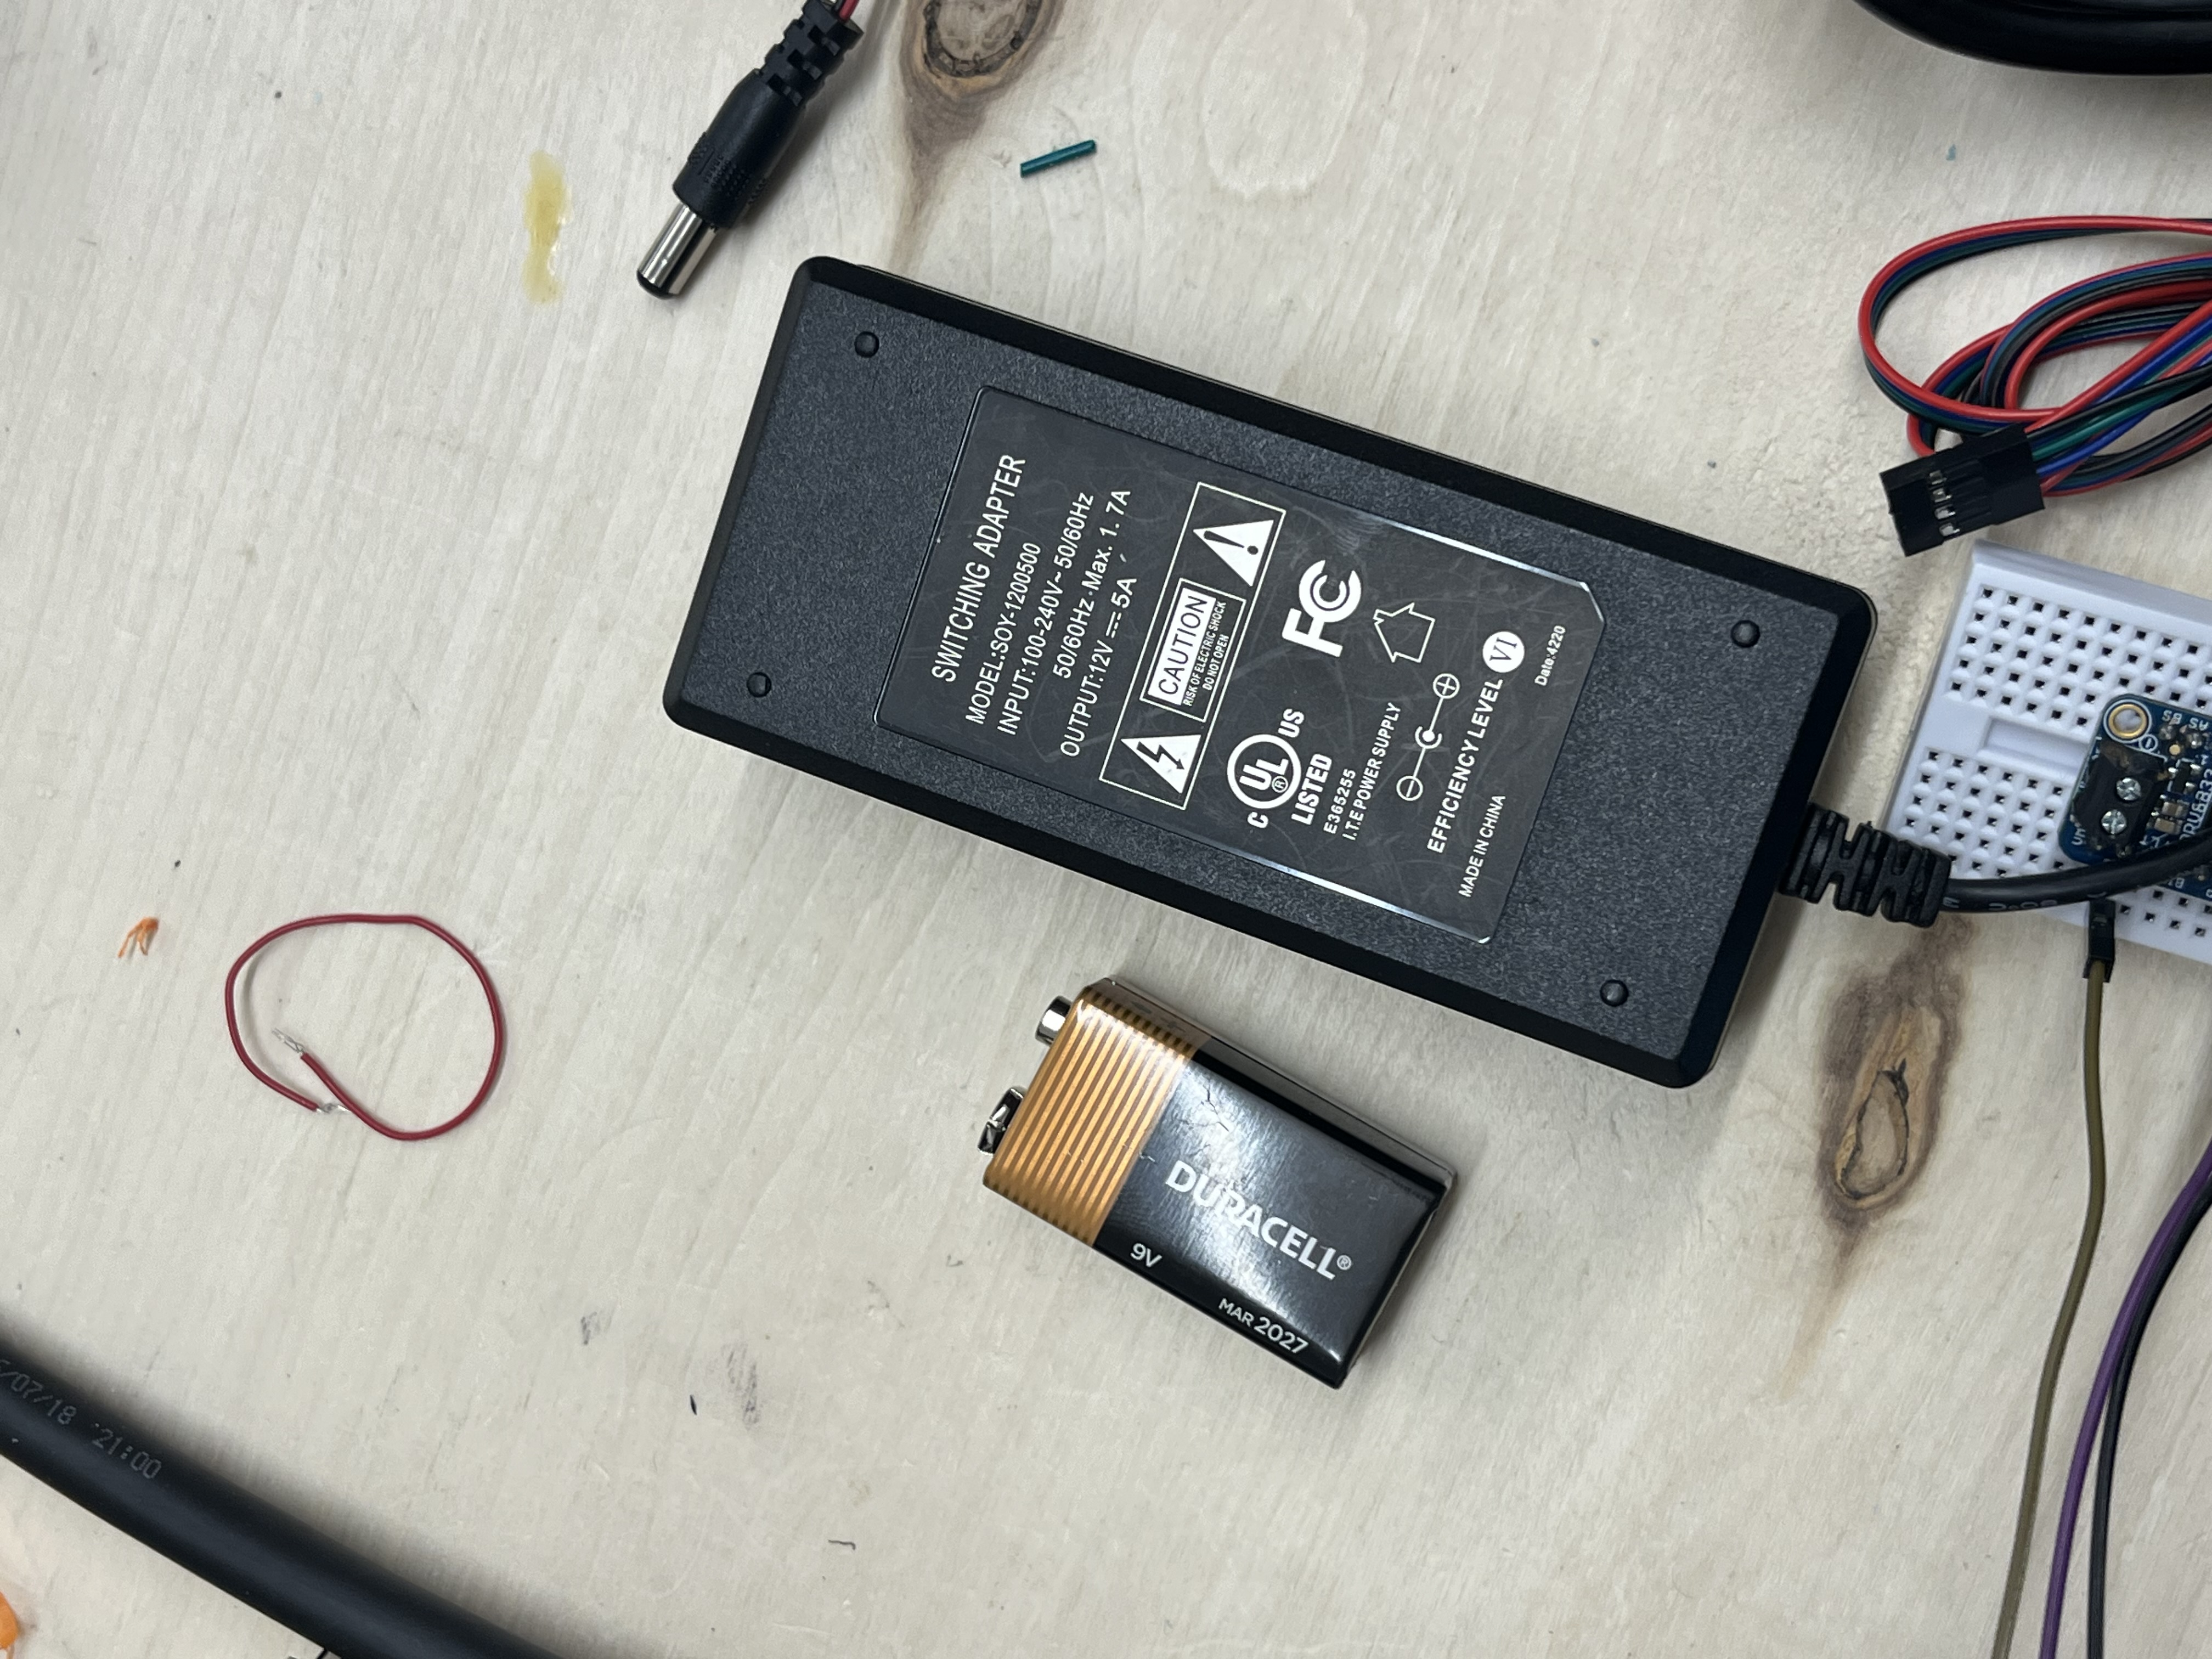
\includegraphics[width=\textwidth, height=2.8cm, keepaspectratio]{DC_Motor_Breadboard_Iteration1.jpeg}\\[2pt]
{\scriptsize Iter.\,1: DC motor + breadboard}
\end{minipage}\hfill
\begin{minipage}[t]{0.30\textwidth}
\centering
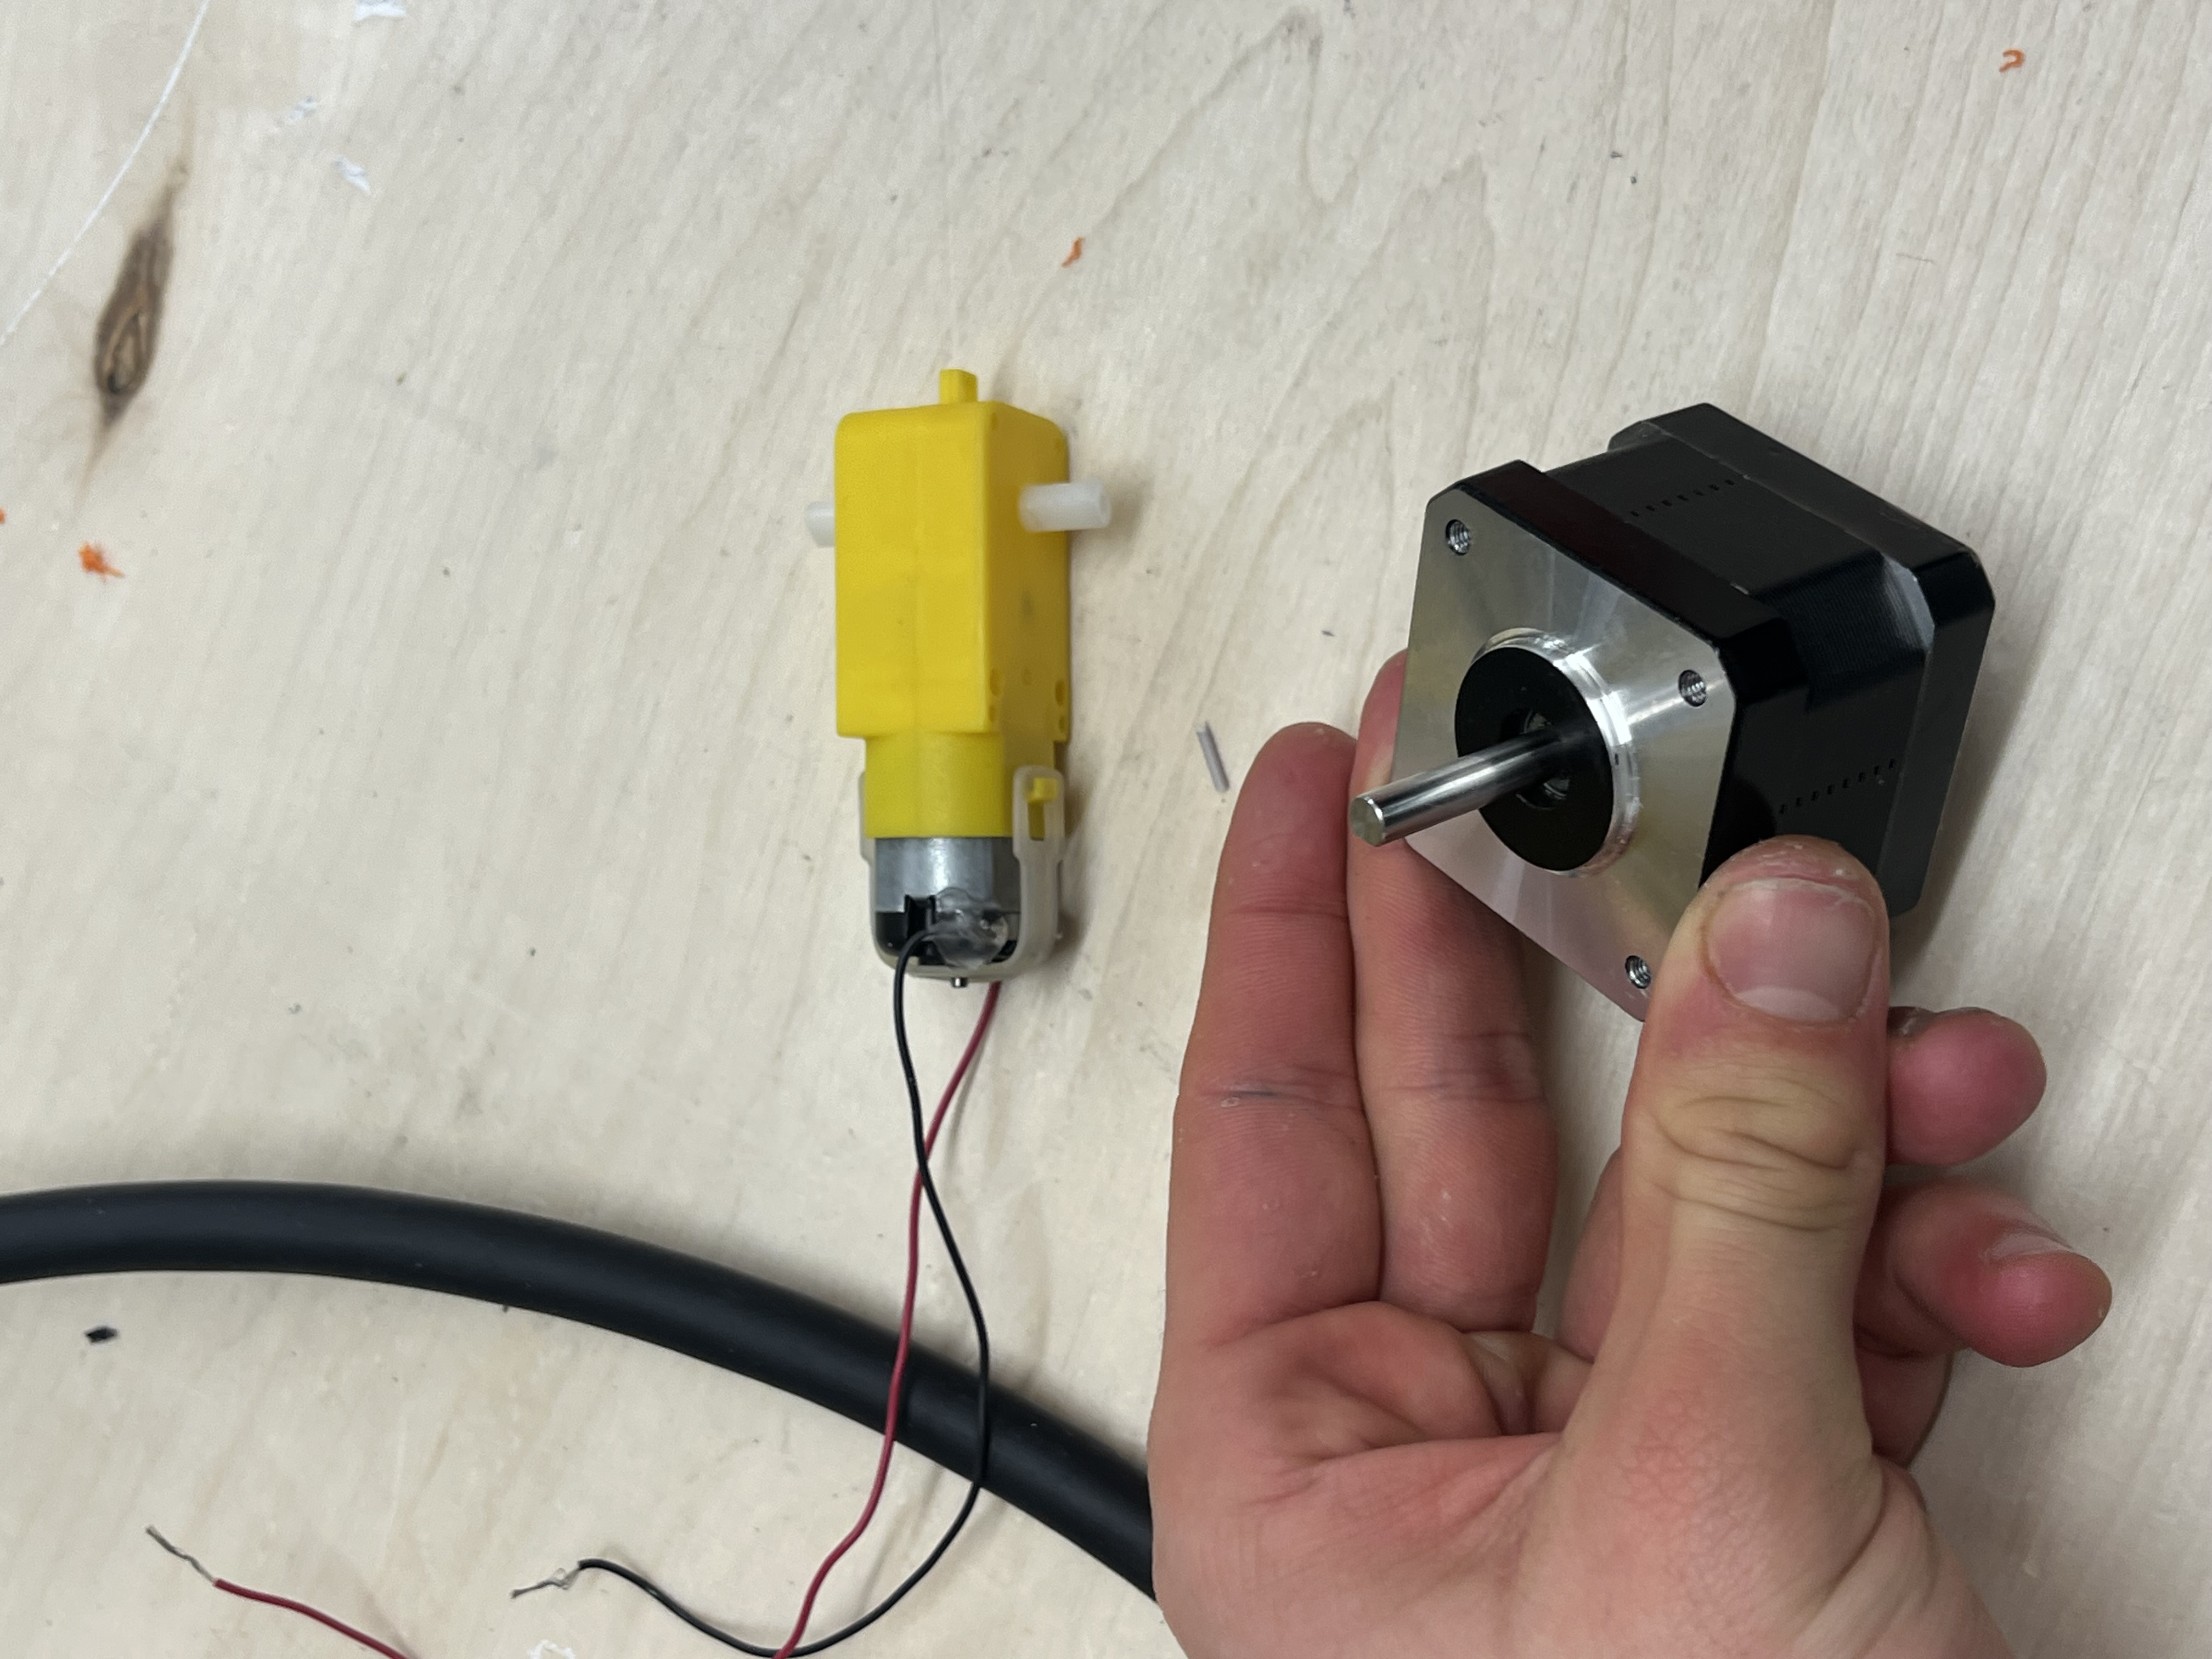
\includegraphics[width=\textwidth, height=2.8cm, keepaspectratio]{HBridge_Motor_Iteration2.jpeg}\\[2pt]
{\scriptsize Iter.\,2: DC motor + H-Bridge}
\end{minipage}\hfill
\begin{minipage}[t]{0.30\textwidth}
\centering
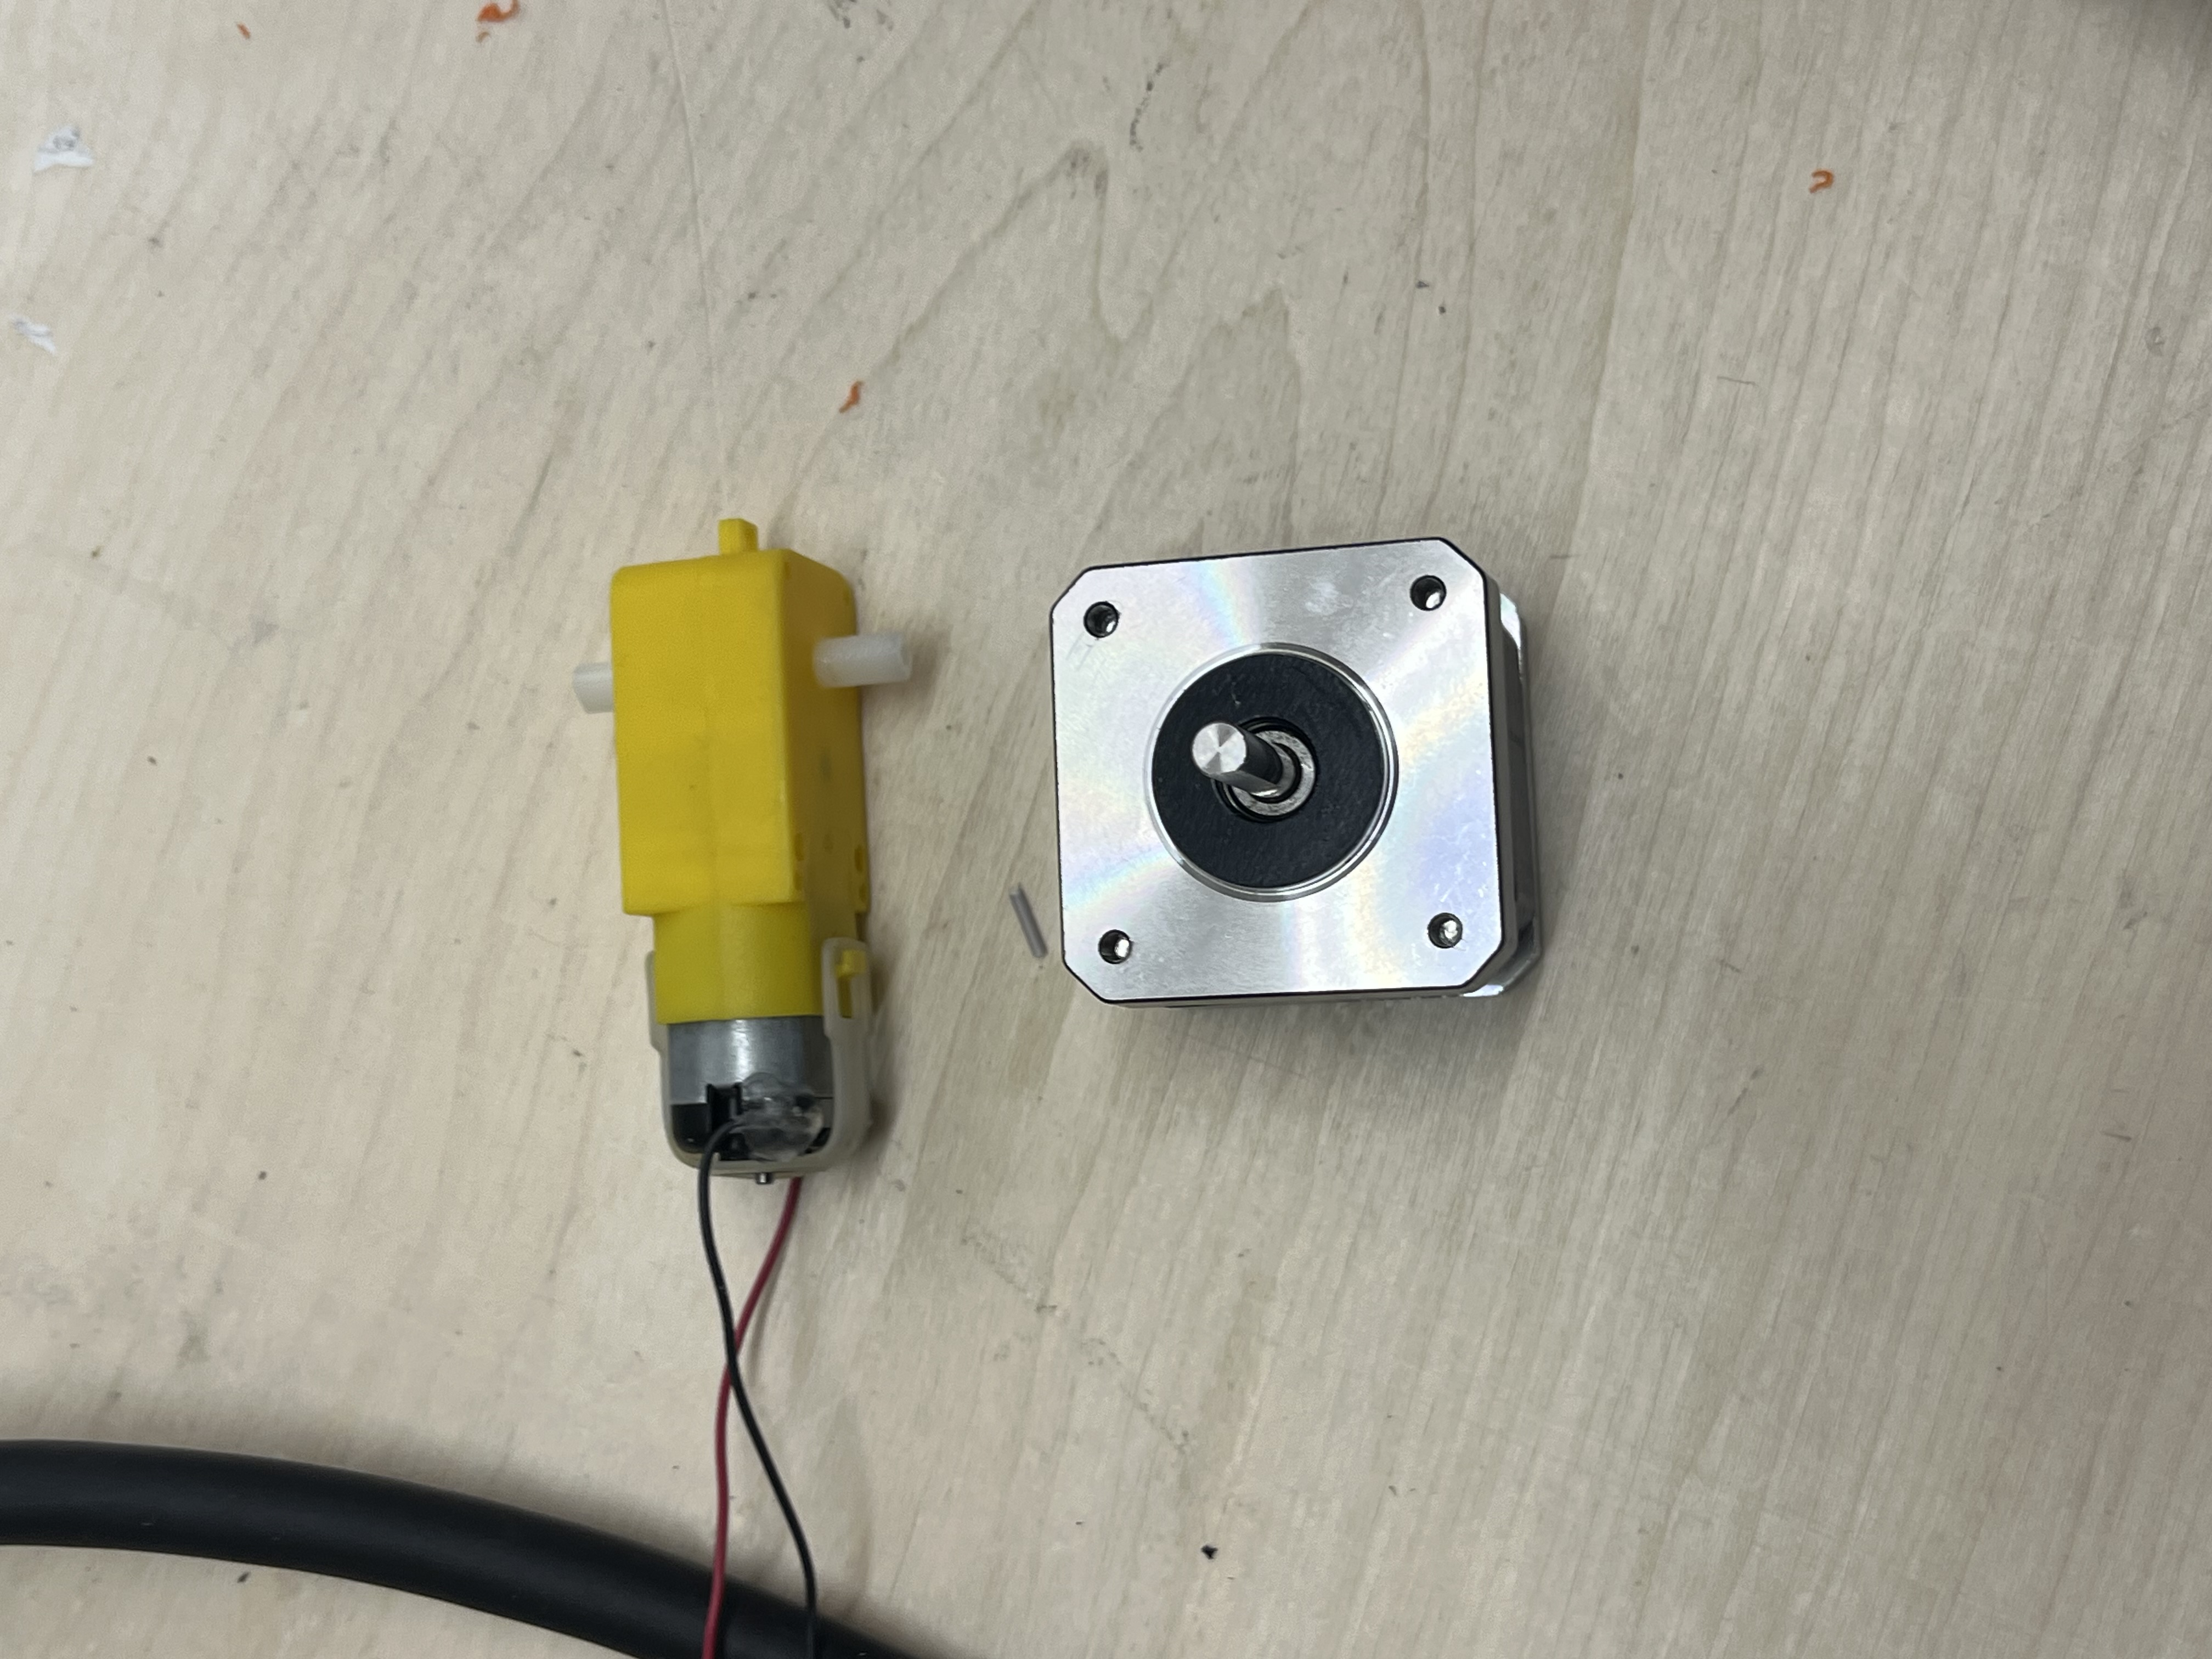
\includegraphics[width=\textwidth, height=2.8cm, keepaspectratio]{Stepper_A4988_ScrewTerminals_Final.jpeg}\\[2pt]
{\scriptsize Final: Nema\,17 + A4988}
\end{minipage}
\caption{Electrical subsystem evolution across three integration iterations.}
\end{figure}

\textbf{Verification of Integration Success:} The 2-minute continuous endurance test confirmed all integration issues were fully resolved. The carriage traversed the full 60\,cm track with zero stalling, the belt maintained tension during direction reversals, and the A4988 remained within safe thermal limits throughout.

\textit{Endurance Test Video:} \href{https://drive.google.com/drive/folders/1wNK_jYUvHXoMne_cIdYbAIURdvYpuG-J}{[Google Drive --- 2-Minute Cycle]}

\end{document}
